\chapter{Aeronautical limitation surfaces}

	\section{Physical limitation surfaces}
	\paragraph{} As runaway 1 and 2 are both classified as category 4, the dimensions of the Aeronautical Servitudes are the same for both. Using the defined OBSTACLE LIMITATION SURFACES (figure \ref{servitudeMap}), on ATTACHMENT B of \cite{Standards2016}.
	
	\begin{figure}[H]
		\centering
		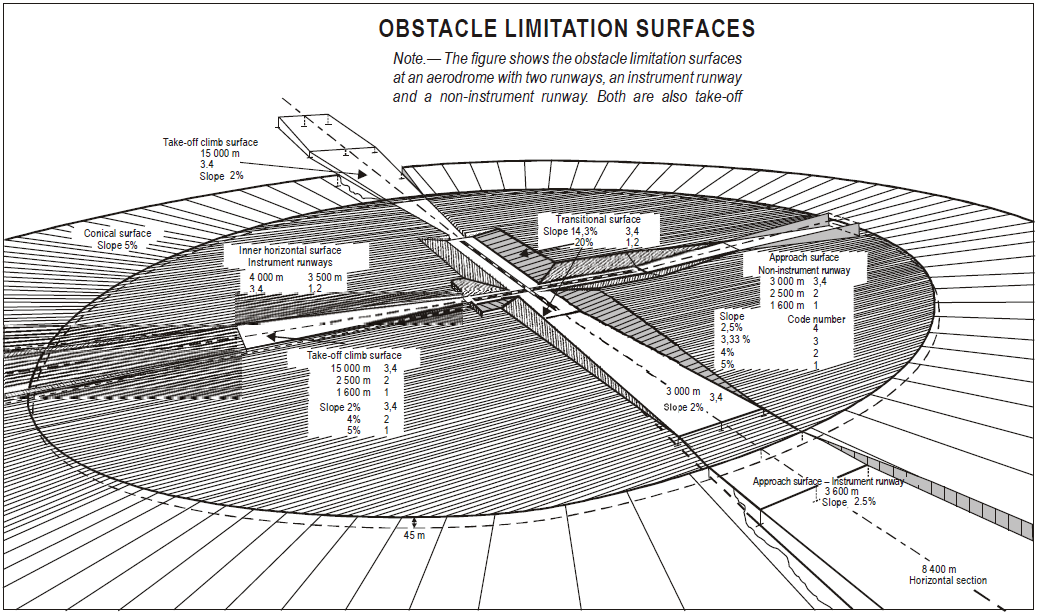
\includegraphics[clip, trim=0cm 0cm 0cm 0cm, width=\textwidth]{./images/servidumbres/servitudeMap}
		\caption{Obstacle Limitation Surface model.}
		\label{servitudeMap}
	\end{figure}

	The servitudes for each runway are determined on the following table and represented on figure \ref{3Dservidumbres}.
	
	%AFEGIR TAULA
	\begin{longtable}[htb]{@{}lr@{}}
		\toprule[3pt]
		\multicolumn{2}{c}{\textbf{\large RUNWAYS 1 \& 2  } }\\ \midrule[2pt]
		\multicolumn{2}{c}{\textbf{Conic} }\\
		\midrule[0.5pt]
		Slope & 5\%\\
		Height & 100m\\
		\midrule[2pt]
		\multicolumn{2}{c}{\textbf{Internal Horizontal} }\\
		\midrule[0.5pt]
		Height & 45m\\
		Radius & 4.000m\\
		\midrule[2pt]
		\multicolumn{2}{c}{\textbf{Internal Approximation} }\\
		\midrule[0.5pt]
		Width & 120m\\
		Distance from edge & 60m\\
		Length & 900m\\
		Slope & 2\% \\
		\midrule[2pt]
		\multicolumn{2}{c}{\textbf{Approximation} }\\
		\midrule[0.5pt]
		Inner band length & 300m\\
		Distance from edge & 60m\\
		Divergence & 15\% \\
		\midrule[0.5pt]
		\multicolumn{2}{c}{First section} \\
		\midrule[0.5pt]
		Length & 3.000m\\
		Slope & 2\%\\
		\midrule[0.5pt]
		\multicolumn{2}{c}{Second section} \\
		\midrule[0.5pt]
		Length & 3.600m\\
		Slope & 2.5\%\\
		\midrule[0.5pt]
		\multicolumn{2}{c}{Horizontal section} \\
		\midrule[0.5pt]
		Length & 8.400m\\
		Total length & 15.000m\\
		\midrule[2pt]
		\multicolumn{2}{c}{\textbf{Transition} }\\
		\midrule[0.5pt]
		Slope \& 14.3\%\\
		\midrule[2pt]
		\multicolumn{2}{c}{\textbf{Inner Transition} }\\
		\midrule[0.5pt]
		Slope & 33.3\%\\
		\midrule[2pt]
		\vspace{5cm}&\vspace{5cm}\\
		\midrule[2pt]
		\multicolumn{2}{c}{\textbf{Interrupted Landing} }\\
		\midrule[0.5pt]
		Inner band length & 120m\\
		Distance from edge & 1800m\\
		Divergence & 10\%\\
		Slope & 3.3\%\\
		\midrule[2pt]
		\multicolumn{2}{c}{\textbf{Take-off Climb} }\\
		\midrule[0.5pt]
		Inner band length & 180m\\
		Distance from edge & 60m\\
		Divergence & 12.50\%\\
		Final width & 1.200m\\
		Length & 15.000m\\
		Slope & 2\% (a)\\
		\bottomrule[3pt]
		\caption{Runways 1 \& 2 servitudes. (a): It is recommended to limit the presence of new objects to a surface with a slope of 1.6\%}
	\end{longtable}
	
	The obstacle free surfaces are the same for the two runways, since they are both of category III. All the data in the table is required in order to achieve this category of precision approximation.
	
	After study of the terrain, it is concluded that there are no obstacles in inside the surfaces. The control tower is below the conic surface as well.
	
	
	\begin{figure}[H]
		\centering
		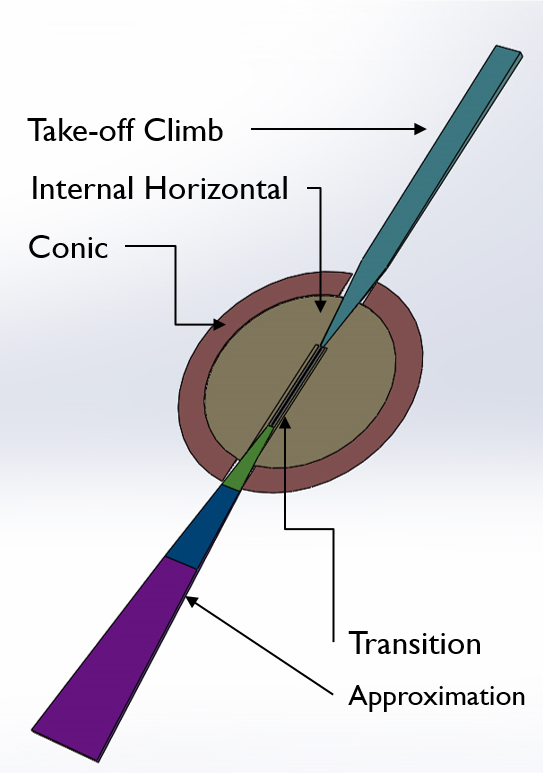
\includegraphics[clip, trim=0cm 0cm 0cm 0cm, width=0.45\textwidth]{./images/servidumbres/3Dservidumbres}
		\caption{Servitudes 3D view.}
		\label{3Dservidumbres}
	\end{figure}

	
	\section{ILS limitation surfaces}
		\section{Localizer limitation surfaces}
		\section{Gliding trajectory protection limitation surfaces}